% Chapter 2: Background and problem characterization.
% Sources: docs/Motivation.txt and docs/research-context.md.

\providecommand{\deadline}{\ensuremath{D}}
\providecommand{\queuewait}{\ensuremath{q}}
\providecommand{\dur}{\ensuremath{T}}
\providecommand{\admitted}{\ensuremath{A}}

\section{Background and Problem Characterization}\label{sec:background}

\subsection{Draft Delivery and Deferred Processing}\label{sec:draft-background}

One shutter event produces multiple buffers that the full post-processing
path collects, fuses, encodes, and saves. The companion Draft path selects its
input earlier, publishes a media-database entry, and retains a recovery image;
the final result later replaces that entry. These paths were designed
together, but the work inside the Draft changed. An effect-free Draft first
gained single-frame Filter and Watermark to resemble the final image. The next
attempted extension was lightweight multi-frame Draft Bokeh for portrait
capture.

Figure~\ref{fig:draft-pipeline} explains why this richer Draft became
necessary. Increasingly expensive processing competes with foreground preview
and capture preparation, so selected modes wait for the application to enter
the background before final composition. Portrait originally composed in the
foreground despite its high cost and large before--after difference. Draft
Bokeh was intended to provide an approximate portrait during this interval and
thereby enable the heavy final portrait composition to be deferred. Repeated
Capture Timeout blocked this transition in two flagship generations.

\begin{figure}[t]
  \centering
  % Companion draft and final paths in the camera post-processing pipeline.
% Included from _2_preliminary.tex.
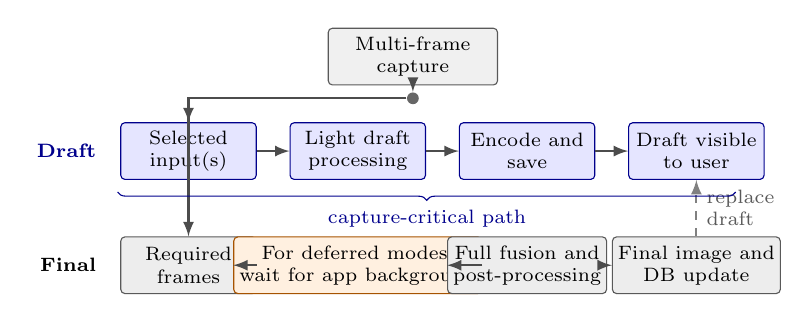
\begin{tikzpicture}[
  font=\scriptsize,
  >=latex,
  box/.style={draw=black!65, rounded corners=1.5pt, align=center,
    minimum width=1.72cm, minimum height=0.72cm, inner sep=2pt},
  draft/.style={box, draw=blue!55!black, fill=blue!10},
  final/.style={box, draw=black!65, fill=gray!14},
  gate/.style={box, draw=orange!65!black, fill=orange!12},
  flow/.style={->, thick, black!70},
  split/.style={circle, fill=black!60, inner sep=1.5pt}
]

  \node[box, fill=black!6, minimum width=2.15cm] (capture) at (3.85,3.55)
    {Multi-frame\\capture};
  \node[split] (fork) at (3.85,3.02) {};
  \draw[flow] (capture) -- (fork);

  % Draft lane.
  \node[anchor=east, font=\scriptsize\bfseries, text=blue!55!black]
    at (-0.05,2.35) {Draft};
  \node[draft] (dinput) at (1.00,2.35) {Selected\\input(s)};
  \node[draft] (deffect) at (3.15,2.35) {Light draft\\processing};
  \node[draft] (dsave) at (5.30,2.35) {Encode and\\save};
  \node[draft] (dvisible) at (7.45,2.35) {Draft visible\\to user};

  \draw[flow] (fork) -| (dinput.north);
  \draw[flow] (dinput) -- (deffect);
  \draw[flow] (deffect) -- (dsave);
  \draw[flow] (dsave) -- (dvisible);

  % Final lane.
  \node[anchor=east, font=\scriptsize\bfseries] at (-0.05,0.90) {Final};
  \node[final] (finput) at (1.00,0.90) {Required\\frames};
  \node[gate] (fgate) at (3.15,0.90) {For deferred modes:\\wait for app background};
  \node[final] (fprocess) at (5.30,0.90) {Full fusion and\\post-processing};
  \node[final] (fupdate) at (7.45,0.90) {Final image and\\DB update};

  \draw[flow] (fork) -| (finput.north);
  \draw[flow] (finput) -- (fgate);
  \draw[flow] (fgate) -- (fprocess);
  \draw[flow] (fprocess) -- (fupdate);

  % The final result replaces the published draft entry.
  \draw[flow, dashed, black!50] (fupdate.north) -- (dvisible.south)
    node[midway, right, align=left, text=black!65] {replace\\draft};

  \draw[decorate, decoration={brace, mirror, amplitude=3pt}, blue!55!black]
    (0.10,1.83) -- (7.95,1.83);
  \node[anchor=north, text=blue!55!black] at (4.03,1.72)
    {capture-critical path};

\end{tikzpicture}

  \caption{Intended portrait transition: Draft Bokeh places a lightweight
  approximation on the deadline-critical Draft path, permitting heavy final
  composition to wait for the application background. $D$ marks the Draft
  delivery deadline.}
  \label{fig:draft-pipeline}
\end{figure}

\subsection{Parallel Capture Turns Latency into Backlog}\label{sec:timeout}

\emph{Capture Timeout} occurs when capture processing, including Draft
delivery, misses the framework's fixed 7-second deadline \deadline. Parallel
capture changed how that deadline is consumed. The HAL may issue
\texttt{captureAvailable} before the preceding Draft completes, allowing the
application to start another capture. Draft Sequences nevertheless share a
single worker.

Figure~\ref{fig:overlap} shows the result. The Draft for capture $i{+}1$ waits
behind capture $i$'s Draft, and the Draft for capture $i{+}2$ waits behind
both. Because each deadline starts at its capture rather than at its Draft
execution, queueing removes budget before any work for that image begins. One
tail-latency spike can therefore cause a later capture to time out even when
every capture executes the same stages.

\begin{figure}[t]
  \centering
  \resizebox{\columnwidth}{!}{% Timeline of two draft sequences overlapping under parallel capture.
% Included from _2_preliminary.tex (Figure~\ref{fig:overlap}).
% Requires: tikz with libraries `patterns' and `decorations.pathreplacing';
% pifont for the check mark.
%
% Design: both captures run the identical stage sequence
% [Bokeh][other][Filter][other][Encode]. Capture i meets its deadline with
% slack; capture i+1 inherits queueing delay from the single draft thread,
% so the same workload overruns its deadline during the mandatory encode.
% Only Bokeh, Filter, and Encode are named; the two remaining draft stages
% are anonymized as short gray "other" stages marked `A' and `B' (their
% durations are small).
\begin{tikzpicture}[font=\small,
  optstage/.style={draw=blue!45!black, fill=blue!14},
  othstage/.style={draw=black!55, fill=gray!22},
  encstage/.style={draw=black!80, fill=black!72},
  queued/.style={pattern=north east lines, pattern color=red!45, draw=red!35},
  ddl/.style={red, dashed, thick}]

  % ---------- legend (top) ----------
  \draw[optstage] (0, 3.2) rectangle (0.3, 3.4);
  \node[anchor=west] at (0.34, 3.3) {\footnotesize optional stage};
  \draw[othstage] (2.45, 3.2) rectangle (2.75, 3.4);
  \node[anchor=west] at (2.79, 3.3) {\footnotesize other stage};
  \draw[encstage] (4.75, 3.2) rectangle (5.05, 3.4);
  \node[anchor=west] at (5.09, 3.3) {\footnotesize mandatory stage};
  \draw[queued] (7.25, 3.2) rectangle (7.55, 3.4);
  \node[anchor=west] at (7.59, 3.3) {\footnotesize queueing delay};

  % ---------- capture i (top row) ----------
  \node[anchor=east] at (-0.2, 2.225) {capture $i$};
  % shutter marker
  \draw[very thick] (0, 1.85) -- (0, 2.6);
  \node[anchor=south] at (0, 2.62) {shutter $i$};
  % lead-in until the draft frame is available
  \draw[densely dotted] (0, 2.225) -- (0.3, 2.225);
  % draft sequence i
  \draw[optstage] (0.3, 2.0) rectangle (1.5, 2.45);
  \node at (0.9, 2.225) {\footnotesize Bokeh};
  \draw[othstage] (1.5, 2.0) rectangle (2.0, 2.45);
  \node at (1.75, 2.225) {\scriptsize\textcolor{black!65}{A}};
  \draw[optstage] (2.0, 2.0) rectangle (2.85, 2.45);
  \node at (2.425, 2.225) {\footnotesize Filter};
  \draw[othstage] (2.85, 2.0) rectangle (3.3, 2.45);
  \node at (3.075, 2.225) {\scriptsize\textcolor{black!65}{B}};
  \draw[encstage] (3.3, 2.0) rectangle (4.15, 2.45);
  \node at (3.725, 2.225) {\footnotesize\textcolor{white}{Encode}};
  % slack before deadline i
  \draw[densely dotted, gray] (4.15, 2.225) -- (6.3, 2.225);
  \node[fill=white, inner sep=1.5pt] at (5.2, 2.225)
    {\footnotesize\textcolor{green!45!black}{\ding{51} in time}};
  % deadline of capture i
  \draw[ddl] (6.3, 1.85) -- (6.3, 2.6);
  \node[red, anchor=south] at (6.3, 2.62) {deadline $i$};

  % ---------- capture i+1 (bottom row) ----------
  \node[anchor=east] at (-0.2, 0.925) {capture $i{+}1$};
  % shutter marker (accepted while draft sequence i is still running)
  \draw[very thick] (1.5, 0.55) -- (1.5, 1.3);
  \node[anchor=south] at (1.5, 1.32) {shutter $i{+}1$};
  % queueing behind draft sequence i
  \draw[queued] (1.5, 0.7) rectangle (4.15, 1.15);
  \node[fill=white, inner sep=1.5pt] at (2.825, 0.925)
    {\footnotesize\textcolor{red!60!black}{queued}};
  % draft sequence i+1 (identical stage durations)
  \draw[optstage] (4.15, 0.7) rectangle (5.35, 1.15);
  \node at (4.75, 0.925) {\footnotesize Bokeh};
  \draw[othstage] (5.35, 0.7) rectangle (5.85, 1.15);
  \node at (5.6, 0.925) {\scriptsize\textcolor{black!65}{A}};
  \draw[optstage] (5.85, 0.7) rectangle (6.7, 1.15);
  \node at (6.275, 0.925) {\footnotesize Filter};
  \draw[othstage] (6.7, 0.7) rectangle (7.15, 1.15);
  \node at (6.925, 0.925) {\scriptsize\textcolor{black!65}{B}};
  \draw[encstage] (7.15, 0.7) rectangle (8.0, 1.15);
  % overrun beyond deadline i+1 (drawn before the label so the text stays visible)
  \draw[draw=red!80!black, fill=red!75] (7.8, 0.7) rectangle (8.0, 1.15);
  \node at (7.575, 0.925) {\footnotesize\textcolor{white}{Encode}};
  % deadline of capture i+1 (crosses the mandatory encode)
  \draw[ddl] (7.8, 0.55) -- (7.8, 1.3);
  \node[red, anchor=south] at (7.8, 1.32) {deadline $i{+}1$};
  % timeout callout
  \node[red!70!black, anchor=west, align=left] at (8.12, 0.925)
    {\footnotesize\bfseries Capture\\[-2pt]\footnotesize\bfseries Timeout};

  % ---------- single-thread handoff ----------
  % Drawn after both rows so the arrowhead is not overpainted by the box
  % borders; the label sits to the right of the arrow.
  \draw[dashed, gray, ->] (4.15, 1.97) -- (4.15, 1.19);
  \node[anchor=west] at (4.27, 1.5)
    {\footnotesize\textcolor{gray}{}};

  % ---------- budget braces ----------
  \draw[decorate, decoration={brace, mirror, amplitude=4pt}]
    (1.5, 0.6) -- (4.15, 0.6);
  \node[anchor=north] at (2.825, 0.38) {\footnotesize budget consumed};
  \draw[decorate, decoration={brace, mirror, amplitude=4pt}]
    (4.15, 0.6) -- (7.8, 0.6);
  \node[anchor=north] at (5.975, 0.38) {\footnotesize remaining budget $b_{i+1}$};

  % ---------- time axis ----------
  \draw[->] (0, -0.4) -- (9.2, -0.4) node[anchor=north east] {time};

\end{tikzpicture}
}
  \caption{Parallel captures queue on one Draft worker. Successive captures
  start Draft execution with less remaining budget until capture $i{+}2$
  reaches its deadline during mandatory encoding.}
  \label{fig:overlap}
\end{figure}

\subsection{Why Level~4 Is Not a Safety Boundary}\label{sec:guard-limit}

The deployed policy originated as an Lv5 response to high-level Draft failures
and was tightened to Lv4 after a lower-tier Filter timeout; shared framework
code applied the same rule to flagships. It disables every optional Draft
stage at Lv4 and above, irrespective of the configured sequence or queue
state. This was a reasonable release safeguard, but
Table~\ref{tab:timeout_index} illustrates its two errors in our motivating
characterization on a flagship device. The table forces the indicated Bokeh
and Filter configurations at every level and reports the first timeout in a
30-shot portrait burst.

% Notes: docs/exhibits.md#tab_timeout_index
\providecolor{tmoS1}{RGB}{252,227,220} %
\providecolor{tmoS2}{RGB}{239,160,140} %
\providecolor{tmoS3}{RGB}{201,80,63}  %
\providecolor{tmoS4}{RGB}{143,36,32}  %

\newcolumntype{H}{>{\centering\arraybackslash}m{1.20cm}}
\newcolumntype{P}{>{\centering\arraybackslash}m{0.67cm}}

\providecommand{\tmoFirst}[2]{\cellcolor{#1}\makebox[\linewidth][r]{#2\hspace{1pt}}}
\providecommand{\tmoFirstW}[2]{\cellcolor{#1}\makebox[\linewidth][r]{\textcolor{white}{\textbf{#2}}\hspace{1pt}}}
\providecommand{\tmoNone}{\makebox[\linewidth][r]{--\hspace{1pt}}}

\begin{table}[t]
 \centering
 \caption{Earliest Timeout onset across capture conditions.}
 \label{tab:timeout_index}
 {\scriptsize\setlength{\tabcolsep}{1.3pt}%
 \begin{tabular}{@{}HPP|PP||PP|PP@{}}
 \toprule
 \multirow[c]{3}{=}[-10pt]{\makecell[c]{\textbf{Starting}\\\textbf{overheat}\\\textbf{level}}} &
 \multicolumn{4}{c||}{\raisebox{-3pt}{\textbf{Normal capture}}} &
 \multicolumn{4}{c@{}}{\raisebox{-3pt}{\textbf{Memory-pressure capture}}} \\[6pt] \cmidrule(lr){2-5}\cmidrule(l){6-9}
 &
 \multicolumn{2}{c|}{\raisebox{-3pt}{\textbf{12MP}}} &
 \multicolumn{2}{c||}{\raisebox{-3pt}{\textbf{24MP}}} &
 \multicolumn{2}{c|}{\raisebox{-3pt}{\textbf{12MP}}} &
 \multicolumn{2}{c@{}}{\raisebox{-3pt}{\textbf{24MP}}} \\[6pt] \cmidrule(lr){2-3}\cmidrule(lr){4-5}\cmidrule(lr){6-7}\cmidrule(l){8-9}
 & \raisebox{-2pt}{\textbf{M{+}S}} & \raisebox{-2pt}{\textbf{M}} &
 \raisebox{-2pt}{\textbf{M{+}S}} & \raisebox{-2pt}{\textbf{M}} &
 \raisebox{-2pt}{\textbf{M{+}S}} & \raisebox{-2pt}{\textbf{M}} &
 \raisebox{-2pt}{\textbf{M{+}S}} & \raisebox{-2pt}{\textbf{M}} \\[4pt]
 \midrule
 Lv0 &
 \tmoNone & \tmoNone & \tmoFirst{tmoS1}{29} & \tmoNone &
 \tmoNone & \tmoNone & \tmoFirst{tmoS1}{26} & \tmoNone \\
 Lv1 &
 \tmoNone & \tmoNone & \tmoFirst{tmoS1}{29} & \tmoNone &
 \tmoFirst{tmoS1}{24} & \tmoNone & \tmoFirst{tmoS2}{19} & \tmoNone \\
 Lv2 &
 \tmoFirst{tmoS1}{24} & \tmoNone & \tmoFirst{tmoS2}{18} & \tmoNone &
 \tmoFirst{tmoS2}{15} & \tmoFirst{tmoS1}{29} &
 \tmoFirst{tmoS2}{14} & \tmoFirst{tmoS1}{25} \\
 Lv3 &
 \tmoFirst{tmoS2}{13} & \tmoFirst{tmoS1}{21} &
 \tmoFirst{tmoS2}{12} & \tmoFirst{tmoS1}{20} &
 \tmoFirstW{tmoS3}{8} & \tmoFirst{tmoS2}{19} &
 \tmoFirstW{tmoS4}{5} & \tmoFirst{tmoS2}{13} \\
 \midrule
 Lv4 &
 \tmoFirstW{tmoS3}{8} & \tmoFirst{tmoS2}{16} &
 \tmoFirstW{tmoS3}{7} & \tmoFirst{tmoS2}{13} &
 \tmoFirstW{tmoS3}{6} & \tmoFirst{tmoS2}{13} &
 \tmoFirstW{tmoS4}{3} & \tmoFirstW{tmoS3}{7} \\
 Lv5 &
 \tmoFirstW{tmoS3}{8} & \tmoFirst{tmoS2}{12} &
 \tmoFirstW{tmoS3}{8} & \tmoFirst{tmoS2}{12} &
 \tmoFirstW{tmoS4}{4} & \tmoFirstW{tmoS3}{9} &
 \tmoFirstW{tmoS4}{4} & \tmoFirstW{tmoS3}{9} \\
 Lv6 &
 \tmoFirstW{tmoS3}{7} & \tmoFirst{tmoS2}{11} &
 \tmoFirstW{tmoS3}{7} & \tmoFirst{tmoS2}{11} &
 \tmoFirstW{tmoS4}{3} & \tmoFirstW{tmoS3}{6} &
 \tmoFirstW{tmoS4}{3} & \tmoFirstW{tmoS3}{6} \\
 \bottomrule
 \end{tabular}%
 }
 \par\vspace{3pt}
 {\scriptsize\begin{minipage}{0.933\columnwidth}
 \raggedright\setlength{\fboxsep}{1.8pt}%
 Earliest timeout onset:~%
 \colorbox{tmoS1}{\strut\,${\geq}\,20$\,}\colorbox{tmoS2}{\strut\,10--19\,}\colorbox{tmoS3}{\strut\,\textcolor{white}{6--9}\,}\colorbox{tmoS4}{\strut\,\textcolor{white}{${\leq}\,5$}\,}\par
 \end{minipage}}
\end{table}

First, the guard is \emph{under-protective}. Bokeh with Filter times out below
the boundary---at Lv0 for 24MP normal capture and Lv2 for 12MP normal capture.
Second, it is \emph{over-restrictive}. At Lv4, the 12MP normal trace completes
nine shots with both stages and 15 with Bokeh alone before its first timeout;
the guard would nevertheless skip optional work even for the first capture.
Overheat correlates with slowdown, but it does not encode image size, memory
pressure, workload composition, or burst backlog. No nontrivial thermal
threshold separates safe and unsafe executions in this characterization.

\subsection{Two Complementary Control Points}\label{sec:control-problem}

Let capture $i$ begin at $a_i$ and its Draft start at $s_i$, giving queueing
delay $\queuewait_i=s_i-a_i$. If $\admitted_i$ is its selected optional work,
$\dur_i(\admitted_i)$ is the duration of the resulting Draft sequence,
including all non-optional work and mandatory encoding. The deadline condition
is

\begin{equation}
  \queuewait_i + \dur_i(\admitted_i) \leq \deadline.
  \label{eq:draft-deadline}
\end{equation}

Admission controls $\dur_i(\admitted_i)$ for the current capture, but cannot
recover budget already lost to $\queuewait_i$. Pacing delays the earliest next
capture opportunity so queued work can drain, reducing future queueing at the
cost of responsiveness; it cannot prevent a tail spike after release. Meeting
all three objectives therefore calls for both controls: avoid timeout, retain
the preferred Draft path when feasible, and minimize added pacing. The next
section presents the shared tail model and the two decisions built on it.
